%              Romero2011hashtag exposure curve -- we find a new
%              mechanism for reducing persistence

In the following sections, we subdivide our analysis of $P(u \mbox{
likes } i | i \in L_{G,C})$ according to three dimensions: social
interaction properties, interest and history user traits, and user
demographic data.  All restrictions on $L$,$G$, and $C$ referenced
below have been defined in Section~\ref{sec:methodology}.  

\subsection{Predictiveness of Interactions}

\label{sec:interactions}

%%%%%%%%%%%%%%%%%%%%%%%%%%%%%%%%%%%%%%%%%%%%%%%%%%%%%%%%%%
\begin{figure*}[t!]
\centering
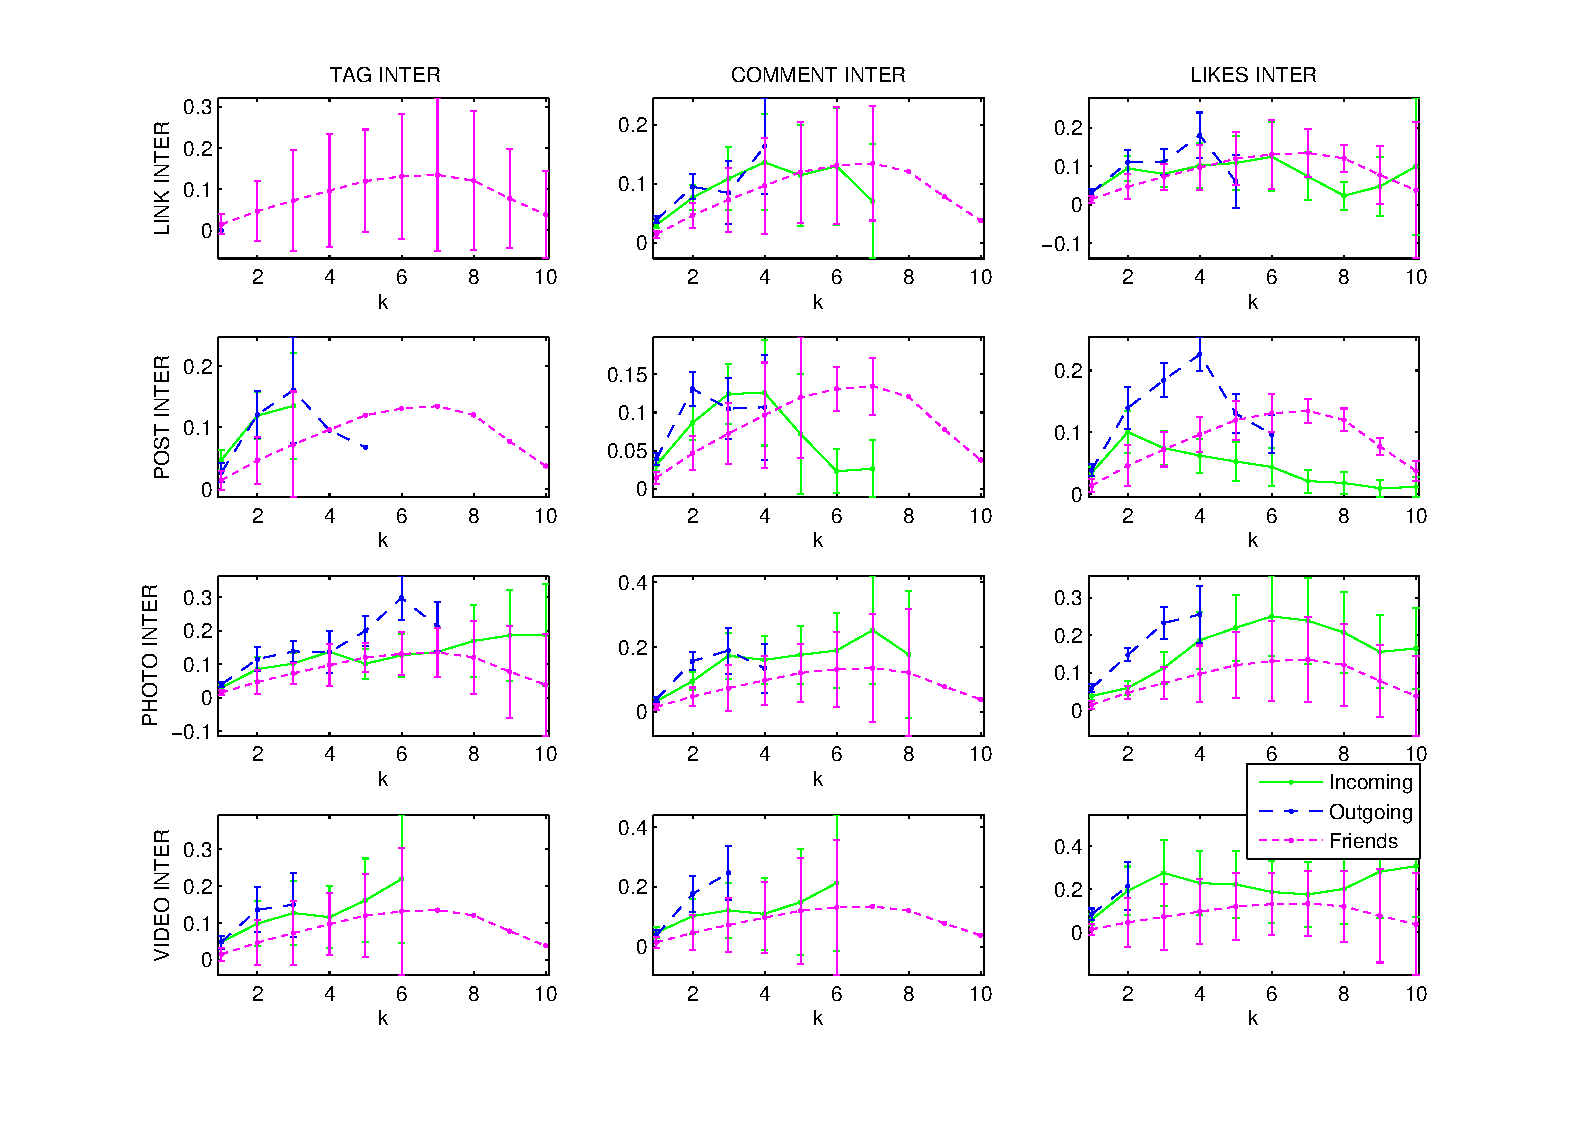
\includegraphics[scale=0.70]{data/likes_vs_inter_fix}
\vspace{-15mm}
\caption{All graphs plot $P(u \mbox{ likes } i | i \in L_{G,C})$
vs. the link criteria that at least $k$ members of $G$ liked item $i$.
The columns restrict $G$ to different 
\textit{Interaction Actions} and the rows restrict $G$ to
different \textit{Interaction Modalities}.  Per graph, each line 
analyzes a different \textit{Interaction Directionality} with
a baseline comparison to groups defined by friends.}
\label{fig:res2}
\end{figure*}
%%%%%%%%%%%%%%%%%%%%%%%%%%%%%%%%%%%%%%%%%%%%%%%%%%%%%%%%%%

In Figure~\ref{fig:res2}, we plot the exposure curves for 
all liked items w.r.t.\ different \textit{Interaction Actions},
\textit{Interaction Modalities}, and
\textit{Interaction Directionality}.  A few important points
are worth noting:
\begin{itemize}
\item As in~\cite{Romero2011hashtag}, we note a saturation
effect as the number of a times an item has been liked
increases, i.e., the curves often peak around 6--8 interactions
then fall off.  
While Romero {\it et al} noted that the
peak of the saturation curve was \emph{topic-dependent}, as a novel
observation we note that the peak is \emph{interaction-dependent}.
Indeed, one can clearly see that when defining groups according
to post interactions (of any directionality), the exposure
curve peaks much earlier than the baseline friends group
exposure curve.  One possible explanation for this is that
post interactions increase exposure to content on a friend's
wall (which are not explicitly recorded as likes) and these
implicit unrecorded exposures thereby lead to a perceived
earlier peak as a function of explicit like exposures.
\item As noted by previous work~\cite{saez2011high}, interaction
direction is highly reflective of preferences.  In general,
the interaction groups with the highest overlap of likes
are the \textit{outgoing} interaction groups --- this makes
perfect sense in a social network setting --- one may tend
to like the same things as the people one is most likely
to initiate an interaction with.
\item For this Facebook data, we note that the specific
interactions with highest predictiveness (both by
statistical signficance and the maximum probability)
are \emph{outgoing post tags}, \emph{outgoing photo likes},
\emph{outgoing post likes}, and \emph{outgoing video comments}.
We hypothesize that video comments are more predictive than
other comments since watching a video (in order to comment on it)
indicates a much higher level of interest in a user than other
commenting interactions (link, post, and photo).
\end{itemize}

% - saturation effect, exposure curve
% - earlier saturation for post interactions (*new modality for 
%   reducing persistence -- more exposures b/c interacting on 
%   user's wall)
% - highest / most significant -- outgoing post tags, photo likes, post likes, video comments -- watch
%   *outgoing study

%%%%%%%%%%%%%%%%%%%%%%%%%%%%%%%%%%%%%%%%%%%%%%%%%%%%%%%%%%
%\begin{figure*}[t!]
%\centering
%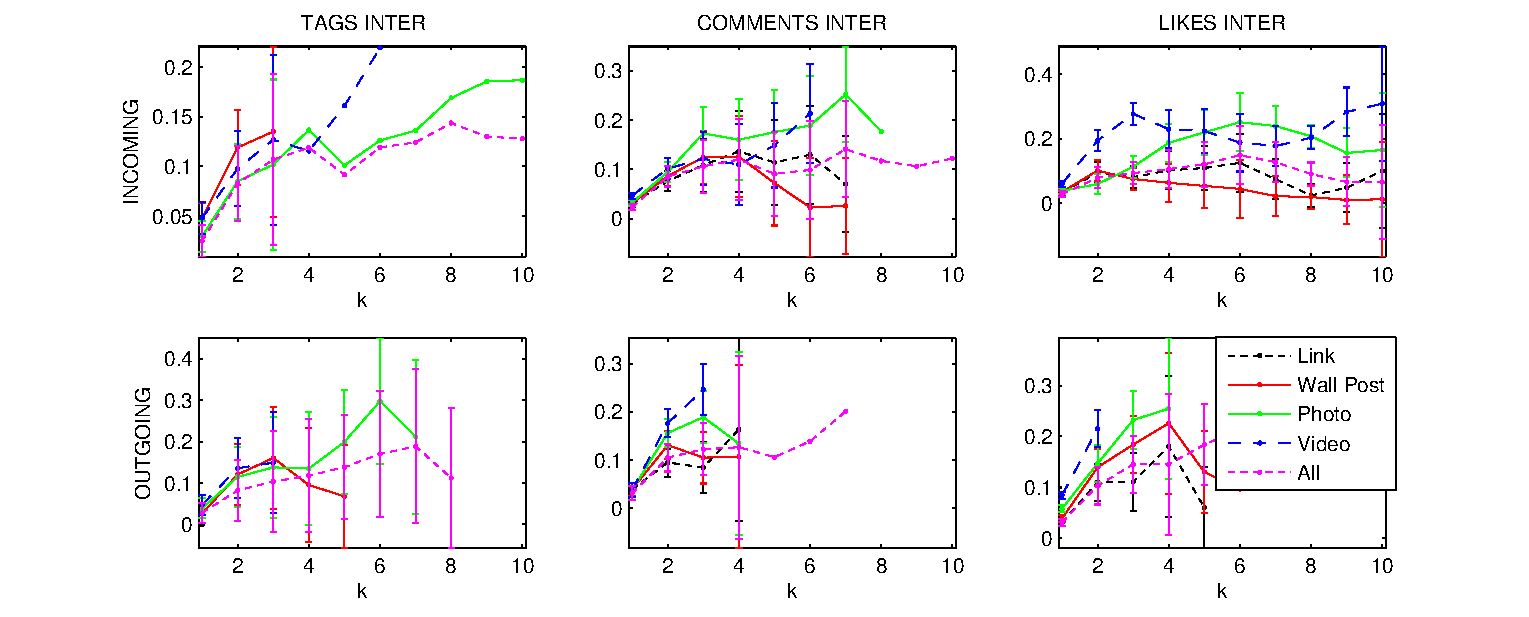
\includegraphics[scale=0.70]{data/dir_vs_lwppv_fix}
%\vspace{-7mm}
%\caption{All graphs plot $P(u \mbox{ likes } i | i \in L_{G,C})$
%vs. the link criteria that at least $k$ members of $G$ liked item $i$.
%The columns restrict $G$ to different 
%\textit{Interaction Actions} and the rows restrict $G$ to
%different \textit{Interaction Directionalities}.}
%\label{fig:res1}
%\end{figure*}
%%%%%%%%%%%%%%%%%%%%%%%%%%%%%%%%%%%%%%%%%%%%%%%%%%%%%%%%%%
%
%In Figure~\ref{fig:res1}
% Come back to this -- basically just outgoing / incoming analysis

%%%%%%%%%%%%%%%%%%%%%%%%%%%%%%%%%%%%%%%%%%%%%%%%%%%%%%%%%%
\begin{figure*}[t!]
\centering
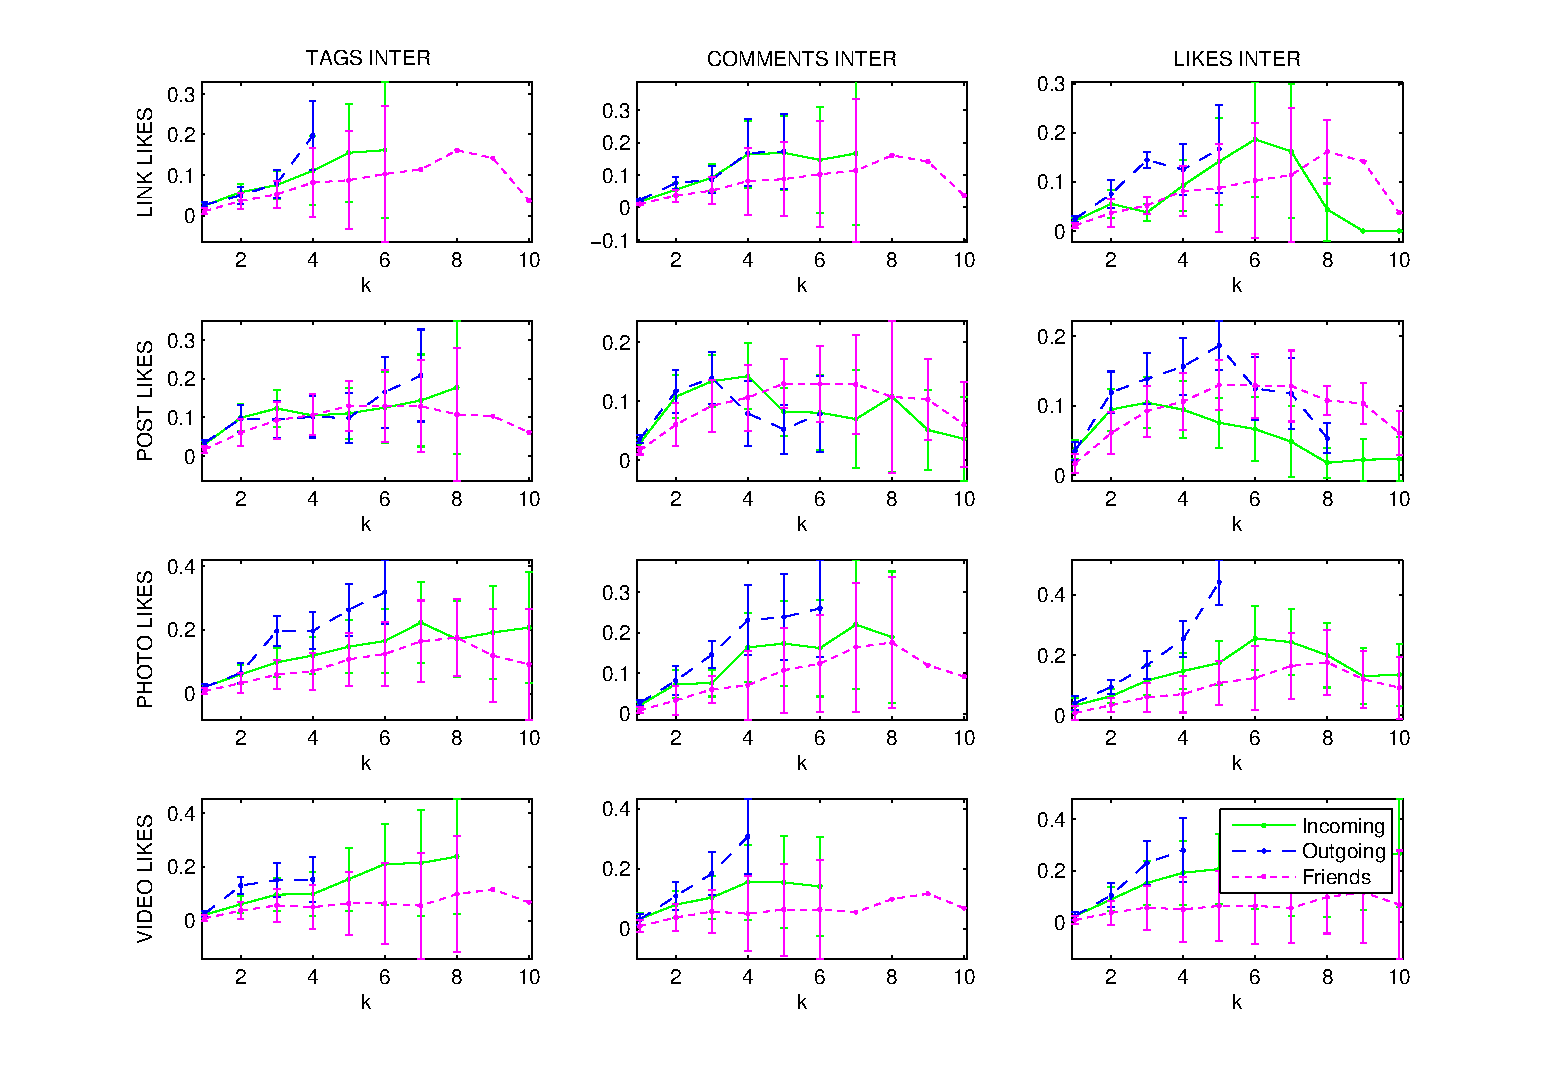
\includegraphics[scale=0.70]{data/linktype_vs_inter_fix}
\vspace{-15mm}
\caption{All graphs plot $P(u \mbox{ likes } i | i \in L_{G,C})$
vs. the link criteria that at least $k$ members of $G$ liked item $i$.
The columns restrict $G$ to different 
\textit{Interaction Actions} and the rows restrict $G$ to
different \textit{Like Types}.    Per graph, each line 
analyzes a different \textit{Interaction Directionality} with
a baseline comparison to groups defined by friends.}
\label{fig:res3}
\end{figure*}
%%%%%%%%%%%%%%%%%%%%%%%%%%%%%%%%%%%%%%%%%%%%%%%%%%%%%%%%%%

In Figure~\ref{fig:res3}, we plot the exposure curves for 
different \textit{Like Types} 
 w.r.t.\ different \textit{Interaction Actions} and
\textit{Interaction Directionality}.  A few important points
are worth noting:
\begin{itemize}
\item For this Facebook data, we note that the specific interactions
with highest predictiveness (both by statistical signficance and the
maximum probability) invariant of the \textit{Like Type} is simply
\emph{outgoing likes}; this seems quite reasonable: users are
likely to like any item liked by users who have posted items they have
liked previously.
\item While all \emph{outgoing interactions} do not predict \emph{post
likes} and \emph{link likes} well, all \emph{outgoing interactions}
appear to predict \emph{photo likes} and \emph{video likes} well.
\end{itemize}
% - all outgoing likes predictive of likes for each individual type
% - outgoing comments mainly predictive for photos and video
% - co-posting groups saturate early

%%%%%%%%%%%%%%%%%%%%%%%%%%%%%%%%%%%%%%%%%%%%%%%%%%%%%%%%%%
\begin{figure*}[t!]
\centering
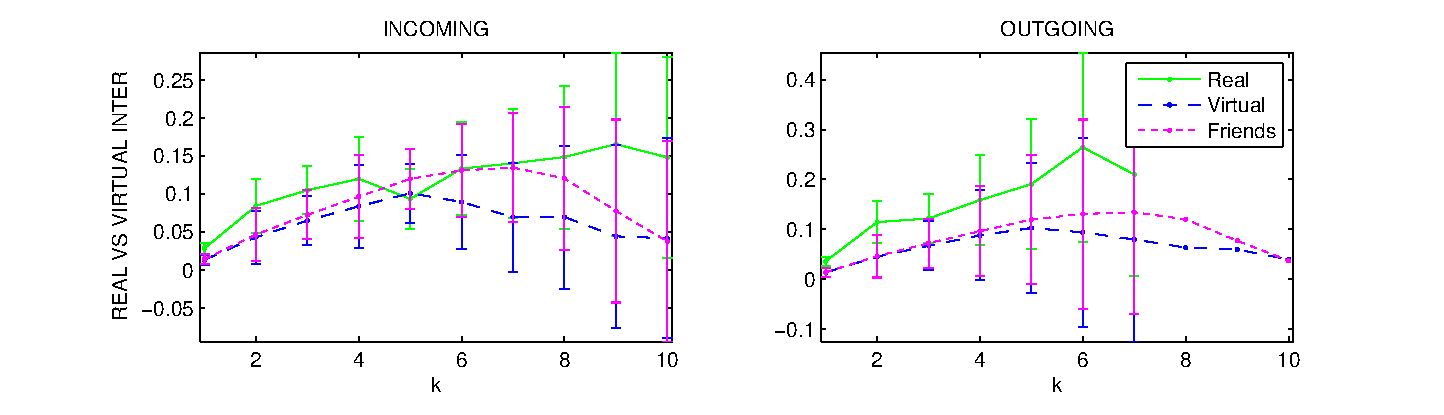
\includegraphics[scale=0.75]{data/real_vs_virtual_fix}
\vspace{-7mm}
\caption{All graphs plot $P(u \mbox{ likes } i | i \in L_{G,C})$
vs. the link criteria that at least $k$ members of $G$ liked item $i$.
The columns restrict $G$ to different 
\textit{Interaction Directionalities}.  Per graph, each line 
analyzes \textit{Real vs. Virtual} with
a baseline comparison to groups defined by friends.}
\label{fig:res4}
\end{figure*}
%%%%%%%%%%%%%%%%%%%%%%%%%%%%%%%%%%%%%%%%%%%%%%%%%%%%%%%%%%

We evaluate in Figure~\ref{fig:res4} which of \emph{incoming} or
\emph{outgoing}, \emph{real} or \emph{virtual} interactions are most
predictive of a user's likes.  In short, while incoming interactions
do not show either real or virtual interacting friends 
to be more predictive of likes than general friends, there is
a stronger trend (although not statistically significant for
any single data point) that \emph{outgoing} interactions for 
\emph{real} friends are more predictive of preferences
than for friends and virtual friends in general. 

\subsection{Predictiveness of User Traits}

\label{sec:interest_history}

While in the previous section we analyzed the predictiveness
of various user interactions, now we analyze the predictiveness
of different user traits.

%%%%%%%%%%%%%%%%%%%%%%%%%%%%%%%%%%%%%%%%%%%%%%%%%%%%%%%%%%
\begin{table*}[t!]
\centering
\begin{tabular}{|c|c|c|} 
\multicolumn{3}{c}{\textbf{$k \geq 1$ Friend Likes}} \\ \hline
& \textbf{Female Friends} & \textbf{Male Friends} \\ \hline
\textbf{Female User} & $0.019 \pm 0.009$ & $0.014 \pm 0.006$ \\ \hline
\textbf{Male User}   & $0.012 \pm 0.003$ & $0.015 \pm 0.009$ \\ \hline
\end{tabular} $\qquad$
\begin{tabular}{|c|c|c|} 
\multicolumn{3}{c}{\textbf{$k \geq 2$ Friend Likes}} \\ \hline
& \textbf{Female Friends} & \textbf{Male Friends} \\ \hline
\textbf{Female User} & $0.085 \pm 0.033$ & $0.059 \pm 0.024$ \\ \hline
\textbf{Male User}   & $0.043 \pm 0.016$ & $0.055 \pm 0.030$ \\ \hline
\end{tabular}
\caption{These two tables plot $P(u \mbox{ likes } i | i \in L_{G,C})$
for different gender demographics where rows indicate the
users $u$ being evaluated and columns indicate the friend groups
being considered.  Results are shown for exposures of both
$k=1$ and $k=2$.}
\label{fig:res6}
\end{table*}
%%%%%%%%%%%%%%%%%%%%%%%%%%%%%%%%%%%%%%%%%%%%%%%%%%%%%%%%%%

Briefly in Table~\ref{fig:res6}, we show predictiveness for
the demographic trait of gender for two exposures.  
While most of these differences are
not statistically significant, both $k=1$ and $k=2$ demonstrate
the same general trend that there is a slight same-gender
preference for item likes in this dataset.

%%%%%%%%%%%%%%%%%%%%%%%%%%%%%%%%%%%%%%%%%%%%%%%%%%%%%%%%%%
\begin{figure*}[t!]
\centering
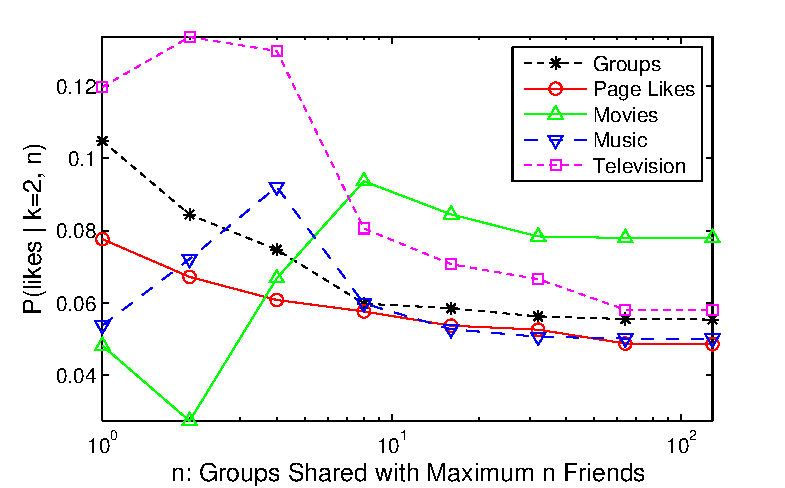
\includegraphics[scale=0.80]{data/interests_fix}
%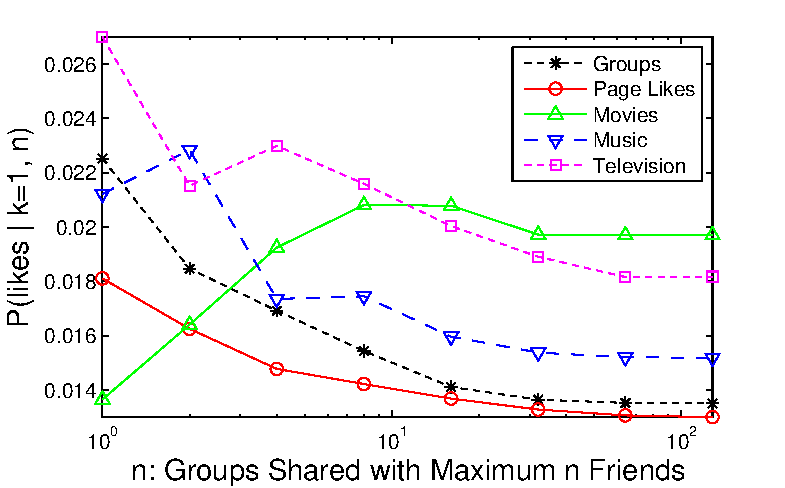
\includegraphics[scale=0.65]{data/interests1_fix} 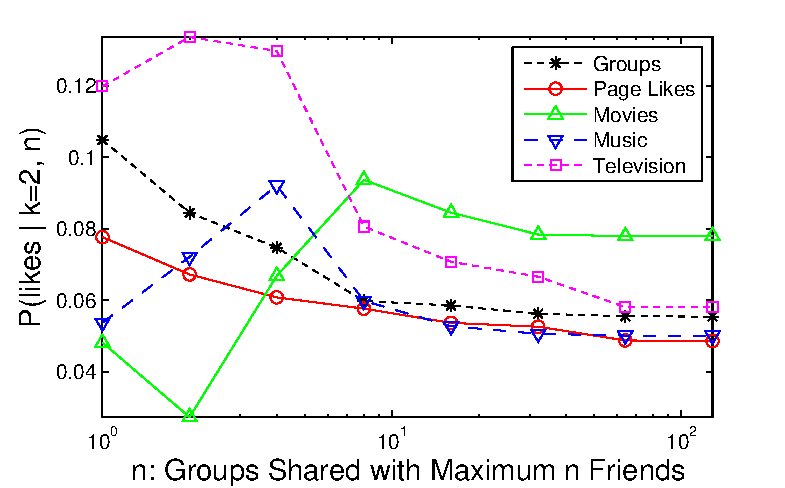
\includegraphics[scale=0.65]{data/interests2_fix}
\vspace{-5mm}
\caption{All graphs plot $P(u \mbox{ likes } i | i \in L_{G,C})$
vs. the link criteria that at least $k$ members of $G$ liked item $i$.
The rows restrict $G$ to different  types of common 
\textit{Interest} or \textit{History} while the columns
indicate exposures of $k=1$ and $k=2$.  Per graph, each line 
analyzes different types of \textit{Interest} or \textit{History}.}
\label{fig:res5}
\end{figure*}
%%%%%%%%%%%%%%%%%%%%%%%%%%%%%%%%%%%%%%%%%%%%%%%%%%%%%%%%%%

In Figure~\ref{fig:res5}, we evaluate the predictiveness of different
types of common \textit{Interest} or \textit{History}.  While none of
these results are statistically significant for any single data point,
there are a number of fascinating trends to observe here:
\begin{itemize}
\item For an exposure of $k=1$ like from different \textit{Interest}
groups, we note that smaller groups are generally more predictive of
user likes than larger groups, which reflects the common sense notion
that large groups appeal more broadly may not be as discriminative of
specific user tastes.  However, it seems this is \emph{not} true for
Movie interests where indeed large groups are more predictive than
similar size groups of other interests. Likewise for \textit{History}
groups, large co-worker groups seem to be more predictive than small
co-worker groups, whereas large groups of schoolmates tend not to be
as predictive.  
%This shows that general
%patterns of interest for \emph{Movies} and \emph{Co-worker} history
%may obey different patterns which makes them predictive in settings
%different from the remaining interests and history.
\item For an exposure of $k=2$ likes, predictiveness of
\textit{Interests} is improved by the general trends from $k=1$
are preserved.  However, it is fascinating to note that 
for \text{History}, the trends are reversed between $k=1$
and $k=2$, with an exposure of $k=2$ for schoolmates indicating
extremely high average predictiveness (above $0.25$, twice
as predictive as any other interest or history displayed).
\end{itemize}
In short, it appears that not all interests and history traits obey
the same trends of predictiveness as a function of group size or
exposure.  On the other hand, the relative predictiveness (or
statistical signficance) of the analysis in this section is somewhat
of a moot point given that the absolute predictiveness of user
interactions from the previous section shows to be much greater (and
statistical signficantly) than any of the user trait analysis in this
section.




